\section{Time Series}

A time series, also known as discrete time signal, is a sequence of observations taken periodically in time. We can use time series to perform many tasks such as predictions of future values, behaviour analysis or information extraction. Examples of time series are audio signals, industrial instrument measures or diary finantial activity.

\begin{figure}[H]
  \centering
  % This file was created with tikzplotlib v0.10.1.
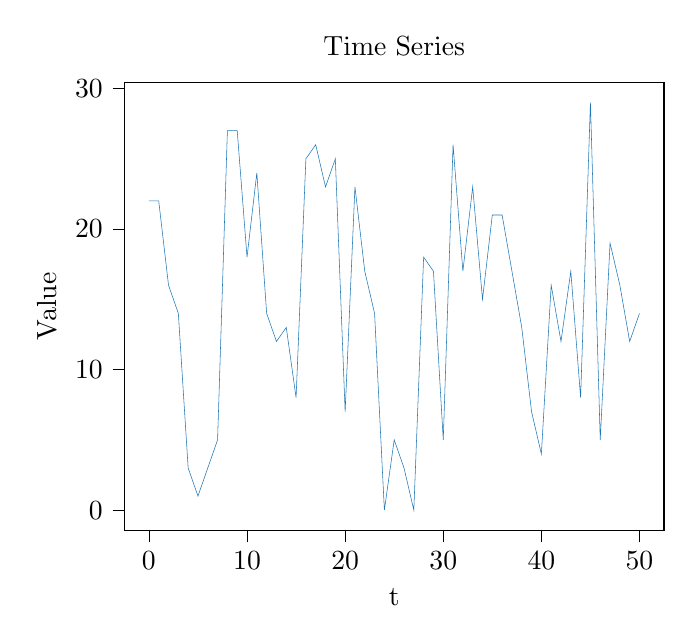
\begin{tikzpicture}

\definecolor{darkgray176}{RGB}{176,176,176}
\definecolor{steelblue31119180}{RGB}{31,119,180}

\begin{axis}[
tick align=outside,
tick pos=left,
title={Time Series},
x grid style={darkgray176},
xlabel={t},
xmin=-2.5, xmax=52.5,
xtick style={color=black},
y grid style={darkgray176},
ylabel={Value},
ymin=-1.45, ymax=30.45,
ytick style={color=black}
]
\addplot [very thin, steelblue31119180]
table {%
0 22
1 22
2 16
3 14
4 3
5 1
6 3
7 5
8 27
9 27
10 18
11 24
12 14
13 12
14 13
15 8
16 25
17 26
18 23
19 25
20 7
21 23
22 17
23 14
24 0
25 5
26 3
27 0
28 18
29 17
30 5
31 26
32 17
33 23
34 15
35 21
36 21
37 17
38 13
39 7
40 4
41 16
42 12
43 17
44 8
45 29
46 5
47 19
48 16
49 12
50 14
};
\end{axis}

\end{tikzpicture}

  \caption{Example of a random time series.}
\end{figure}
A system can be determined comparing the input and the output. We call the system a filter if it is linear and time invariant. Considering the dynamic system as a black box, we can estimate the transference function or the impulse response to taht filter.

We can also consider \textbf{multivariate} time series, where some values of the time series have an influence on the other values in different or the same time instant. We can \textbf{classify} the time series in two wide types:

\begin{itemize}
  \item Determinist: based in dynamic systems, they exploit the phisics of the generation algorithm of the time series.
        \item Stochastic: where the series are realizations of a stochastic process, which can be modelated.
\end{itemize}

In this subject, we will focus on stochastic models.

\subsection{Stochastic Models}

We can make three big considerations on the stochastic models.
\begin{itemize}
  \item Stationary models.
        \begin{ndef}
          Let \(\{X_{t}\}\) be a stochastic process and let \(F_{X}\left(x_{t_{1} + \tau}, \dots, x_{t_{n} +\tau}\right)\) represent the CDF of the \textbf{unconditional} joint distribution of \(\{X_{t}\}\) at times \(t_{1 }+ \tau,\dots, t_{n} + \tau\). Then \(\{X_{t}\}\) is strictly stationary if
          \[
            F_{X}\left( x_{t_{1} + \tau}, \dots, x_{t_{n} +\tau}\right) = F_{X}\left(X_{t_{1}},\dots,x_{t_{n}}\right)
          \]

        \end{ndef}
        However, we will use the case of \textbf{weak stationarity}, where we assume that the expectation of the stochastic process and the covariance at times \(t,t+\tau\) are constant.

        \begin{example}
          AR, MA, ARMA
        \end{example}

  \item Non stationary models, where we do not make the assumption that the average of the process is constant in time and that there is seasonality
        \begin{example}
          ARIMA, SARIMA
        \end{example}

  \item Influenced by exogenous(extern) variables. In this cases, the exogenous variable affects the model, but the model does not affect this variable.
        \begin{example}
          SARIMAX
        \end{example}
\end{itemize}

Let us introduce some \textbf{notation} for the following explanations

\begin{ndef}
  Let \(z_{t}\) be the value of the time series at instant \(t\).
  \begin{itemize}
    \item The \textbf{backward shift} operator is \(z_{t-m} = B^{m}z_{t}\)
    \item The \textbf{forward shift} operator is \(z_{t+m} = F^{m}z_{t} = B^{-m}z_{t}\)
    \item The difference or discrete gradient operator is \(\nabla z_{t} = z_{t} - z_{t-1} = (1-B)z_{t}\)
  \end{itemize}
\end{ndef}

Recall that, having a time series we can consider its \textbf{Z-transform}, that converts the discrete-time signal into a complex frequency-domain representation. In the Z-transform representation, the previously introduced notation is:
\begin{itemize}
  \item The backward shift is \(z_{t-m} = B^{m}z_{t} = Z^{-m}z_{t}\)
  \item The forward shift is \(z_{t+m} = B^{-m}z_{t} = Z^{m}z_{t}\)
        \item The difference or discrete gradient is \(\nabla z_{t} = (1-Z^{-1})z_{t}\)
\end{itemize}


\section{Linear filter based models}

The stochastic models we use are based on time series \(z_{t}\) in which sucessive values are highly dependent. In these cases, we can see that the time series is generated from a series of independependent ``shocks''.

\begin{ndef}
  Let \(a_{t} \sim \mathcal N\left(0,\sigma_{a}^{2}\right)\) be \emph{white noise} (where each \emph{shock} is related to \(a_{t}\)) which is not observed. Consider a linear filter that transforms the unobserved \(a_{t}\) to a observed time series \(z_{t}\). We say that a \textbf{linear filter model is}
  \begin{equation}\label{linear:filter}
    z_{t} = \mu + a_{t} + \psi_{1}a_{t-1} + \psi_{2}a_{t-2} + \dots = \mu + \psi(B)a_{t},
  \end{equation}
  where
  \[
    \psi(B) = 1 + \psi_{1}B + \psi_{2}B^{2} + \dots
  \]
  is called the \textbf{transfer function} of the filter.
\end{ndef}

\begin{figure}[H]

  \centering
  \includegraphics{Figures/LinearFilter}

\end{figure}

As we can see, we are expressing the filter in terms of a infinite sum of the coefficients \(\psi_{i}\). If there are finite coefficients of the sum is \emph{absolutely summable}, that is: \(\sum_{j = 0}^{\infty}\abs{\psi_{j}} < \infty\) or the vector of coefficients has finite \(\ell^{1}\) norm, we say that the filter is \textbf{stable} and the process \(z_{t}\) is \textbf{stationary}.

In the case where the \(\ell^{1}\) norm is not finite, our filter are non-stable and produce non-stationary series.

\subsection{Autoregressive Models (AR)}

Let us firstly consider the simplest case of linear filter. An \textbf{autoregressive model} is a linear filter where the current value of the process \(\tilde z_{t}\) is expressed as a finite sum of the previous values and a random shock \(a_{t}\).

\begin{ndef}
  Let us denote the values of a process af equally spaced times \(t,t-1,\dots\) by \(z_{t}, z_{t-1}, \dots\). Consider that the values are centered, that is \(\tilde z_{t} = z_{t} - \mu\). Then, the \textbf{autoregressive (AR) process} of \textbf{order p} is
  \begin{equation}\label{model:AR}
    \tilde z_{t} = \phi_{1}\tilde z_{t-1} + \phi_{2}\tilde z_{t-2}+ \dots  + \phi_{p}\tilde z_{t-p} + a_{t}
    \end{equation}
\end{ndef}

Note that it is called autoregressive since, if you consider \(\tilde z_{i-k}\) for \(k = 1,\dots,p\) as points, you are doing a \emph{linear regression} over the past values.\\

Now, if we define the \textbf{autoregressive operator of order p} using the backward shift operator \(B\) as:
\[
\phi(B) = 1- \phi_{1}B - \phi_{2}B^{2} - \dots - \phi_{p}B^{p},
\]
we can economically write the autoregressive model in \eqref{model:AR} as
\begin{equation}\label{model:ar:red}
  \phi(B)\tilde z_{t} = a_{t}
\end{equation}

In practice, this model has \(p+2\) unknown parameters \(\mu,\phi_{1},\dots,\phi_{p},\sigma_{a}^{2}\) which have to be estimated from the data.

\begin{nprop}
The autoregressive model is a particula case of a linear filter
\end{nprop}
\begin{proof}
  Although we will not be estrictly formal in this proof, we will give an intuition on the iterative process that has to be done.

  Consider the term \(\tilde z_{t-1}\), let us eliminate it. Recall that
  \[
    \tilde z_{t-1} = \phi_{1}\tilde z_{t-2} + \dots + \phi_{p} \tilde z_{t-p-1} + a_{t-1}.
  \]
  We can substitute this term in the expression of the AR model given in Equation \eqref{model:AR}. The same can be done for \(\tilde z_{t-2}\) and so on, to yield eventually an infinite series in the \(a\) terms.

\end{proof}

  In the case where \(p=1\), we have the AR process \(\tilde z_{t} = \phi \tilde z_{t-1} + a_{t}\). After \(m\) sucessive substitutions of \(\tilde z_{t-j} = \phi \tilde z_{t-j-1} + a_{t-j} \), with \(j = 1,\dots,m\), we obtain
  \[
    \tilde z_{t} = \phi^{m+1}\tilde z_{t-m-1}+ a_{t} + \phi a_{t-1} + \phi^{2}a_{t-2} + \dots + \phi^{m}a_{t-m}
  \]
  Now, if we take the limit \(m\to \infty\) this leads to the \emph{convergent inifinite series representation} \(\tilde z_{t} = \sum_{j=0}^{\infty}\phi^{j}a_{t-j}\), with \(\psi_{j} = \phi^{j}, j \geq 1\), provided that \(\abs{\phi} < 1\). In the general AR case,
  \[
    \phi(B) \tilde z_{t} = a_{t}
  \]
  is equivalent to
  \[
    \tilde z_{t} = \phi^{-1}(B) a_{t} = \psi(B)a_{t}, \quad \quad \psi(B) = \phi^{-1}(B) = \sum_{j=0}^{\infty}\psi_{j}B^{j}.
  \]

  AR processes can be stationary or nonstationary. From the definition, it is clear that for a AR process to be stationary, the coefficients \(\phi\) must be such that the weights \(\psi_{1},\psi_{2},\dots\) in \(\psi(B) = \phi^{-1}(B)\) form a convergent series. A \textbf{necessary requirement} for stationarity is that the autoregressive operator \(\phi(B)\), considered a polynomial in \(B\) of degree \(p\), must have all roots greater than \(1\) in absolute value.

  \subsection{Application: Linear Prediction Coefficients in Speech Coding}


  Let us now set in the case of the \textbf{Speech Coding} topic. It is considered that a speech sample can be approximated as a linear combination of the past samples, which is how an AR model behaves. We have to find the coefficients that best suit our problem, using for instance the mean squared error prediction. We use the obtained \textbf{Linear Prediction Coefficients (LPCs)} to represent the signal frame.

  Using this technique, we would be \textbf{reducing} the signal size significantly. However, since we are only approximating the signal, we would be most probably losing information. Two examples of codification of the audio signals are:

  \begin{itemize}
    \item MP3: which produces a different audio signal, involving loss of information
          \item FLAC: where the output is almost equal to the input, no loss of information
\end{itemize}

Signals are digitalized using a coding system.

\begin{figure}[!h]
  \centering
  \includegraphics[scale=0.5]{Figures/SpeechCodingSystem}
  \caption{Block diagram of a speech coding system.}
\end{figure}

The filter eliminates aliasing and the sampler makes the continuous to discrete time conversion.

\begin{example}
  In this example, we present the digital CD audio signal and why we would like to reduce its size without losing information. This signal has the following properties:

  \begin{enumerate}
    \item Sample rate \(\Omega_{s} = 44.1 kHz\)
    \item Bits per sample: \(16\)
          \item 2 channels (although sometimes 3 are used)
  \end{enumerate}

  With this properties, the input bit rate is
  \[
    R = \Omega_{s} \ \cdot \ \operatorname{Bits/sample} \ \cdot \ \operatorname{Channels} = 44.1*10^{3} * 16 * 2 = 14112000 \frac{\operatorname{bits}}{s} = 1.41 \frac{\operatorname{Mb}}{s}
  \]
  Which implies that, in a single minute we would need
  \[
    60s ; * ; 1,4112 \frac{\operatorname{Mb}}{s} ; * ; \frac{1 \operatorname{byte}}{8 \operatorname{bits}} = 10.09 \operatorname{MB},
  \]
  which is a high size for a single minute audio.
\end{example}

\begin{example}
  In this example, we will present the input bit rate for the speech digital signal. Its common properties are:
    \begin{enumerate}
    \item Sample rate \(\Omega_{s} = 8 ; \operatorname{kHz}\)
    \item Bits per sample: \(16\)
          \item 1 channel
    \end{enumerate}

  With this properties, the input bit rate is \(128\) Kb per second.

\end{example}

As a quick note, remember that \textbf{to quantify} a continuous time series is to assign it discrete amplitude values. When we do this, we are introducing a \textbf{cuantification error},
\[
\operatorname{error}(t) = z_{\operatorname{quantified}}(t) - z_{\operatorname{original}}(t)  
\]
In each \(t \in \mathbb R\), this error can be positive or negative. We can consider that the error is additive.\\

Let us consider a simplified version of the speech production model. Consider that there is a source and a filter, such as in the next figure:

\begin{figure}[!h]
\centering
\includegraphics[scale=0.6]{Figures/SpeechGeneration}
\caption{LPC model of speech production.}
\end{figure}

Then,

\begin{itemize}
  \item We assume that we can separate the voice in non overlapping frames that are short enough to keep the model parameters constant.
  \item Then, we estimate the model parameters for each frame . These parameters are: voicing, gain (energy level of the frame), filter coefficients (response of the synthesis filter), pitch period (time length between consecutive excitation impulses)
\end{itemize}

\subsubsection*{Using the AR model to compute the synthesis filter coefficients}

We can use the autoregressive model to predict a speech sample. Let \(x[n]\) be the discrete signal. The prediction aims to find the coefficients \(a_k\), \(k = 1,\dots, p\) such that we can compute that sample using the previous samples

\[
x[n] \approx \sum_{k=1}^p a_k \ x[n-k] \implies x[n] = \sum_{k=1}^p a_k \ x[n-k] + e[n] = \sum_{k=1}^p a_k \ x[n-k] + Ge'[n],
\]
where \(e[n]\) is the error at time step \(n\), \(e'[n]\) is the theoretical excitation and \(G\) is the gain. We \textbf{minimize the mean squared error}(also called mean energy) of the prediction error \(e[n]\) in order to fit this model.

\section{ARMA, (S)ARIMA(X) and Multivariate series}


In this section we will generalize the Autoregressive model, adding complexity (and thus more generalization capability) to it.

\subsection{MA and ARMA}

Firstly, we bring back the general expression of a linear filter given in Equation \eqref{linear:filter}:
\[
\tilde z_t = a_t + \sum_{j=1}^\infty \psi_j a_{t-j}. 
\]

We can consider a special case when only the first \(q \in \mathbb N\) are nonzero.

\begin{ndef}
A \textbf{Moving Average (MA)} process of order \(q\) is a linear filter where only the first \(q\) terms are nonzero
\begin{equation}\label{model:MA}
\tilde z_t = a_t - \theta_1 a_{t-1} - \dots - \theta_q a_{t-q}.
\end{equation}
\end{ndef}
As it can be appreciated, we now use the symbols \(-\theta_1,\dots, -\theta_q\) for the finite set of \emph{weights}. What we are doing is to \emph{smooth} the white noise \(a_t\).


Recall that, as we did before, we can express the moving average model as
\[
\tilde z_t = (1- \theta_1 B - \theta_2 B^2 - \dots - \theta_q B^q) a_t = \theta(B) a_t.
\]

The Moving Average models are \textbf{not addecuate} when the series has \emph{autocorrelation} (that is, relation to its past values). Also, real-life time series are ``more than white noise'' to smooth.

A solution for this disadvantages could be combining the MA model with the AR model linearly:

\begin{ndef}
The \textbf{Autoregressive-Moving Average (ARMA)} process of order \(p,q\) is defined as a linear combination of both models
\[
\tilde z_t = \sum_{i = 1}^p \phi_i \tilde z_{t-i} + a_t - \sum_{j = 1}^q \theta_j a_{t-j}, 
\]
or 
\[
\phi(B)\tilde z_t = \theta(B)a_t. 
\]
\end{ndef}

Using an ARMA model, we are not only capturing the relationships between a point \(\tilde z_t\) and its previous ones (AR), but also smoothing the influence of the white noise (MA).

A great \textbf{disadvantage} of the ARMA models is that they are \textbf{always stationary}, so we cannot model non-stationary time series.

The following proposition presents a very interesting results on ARMA models:

\begin{nprop}
  An ARMA process is stationary if all the roots of \(\phi(B) = 0\) have module greater than one, and it is (explosive) non stationary if the roots have module lesser than one.

\end{nprop}

The left-to-mention case where the roots of \(\phi(B) = 0\) lie \textbf{on} the unit circle is very interesting. Nonseasonal series are often well represented by models in which one or more roots are unitary.
\section{Non estationarity}

Many time series appearing in real life have non stationary behaviour. Thus, we have to obtain new models to be able to make prediction of future values.

However, we can decompose these time series and treat them separately. 

\begin{figure}[H]
\centering
\includegraphics[scale=0.7]{Figures/Decomp}
\caption{Multiplicative decomposition of a time series.}
\end{figure}



Tipically, we use the following components (all of them at time \(t\)):

\begin{enumerate}
\item \(T_t\), the \textbf{trend} component, reflecting the long-term progression of the series. It exists when there is a persistent increasing or decreasing direction on the data. It is not neccesarily linear.

\item \(S_t\), the \textbf{seasonal} component, reflecting the seasonal variation. A seasonal pattern exists when a time series is influenced by seasonal factors. Seasonality occurs over a fixed known period of time.

\item \(R_t\), the \textbf{residual} component, describing randomness or irregular influences
\end{enumerate}

Ocassionally, an additional cyclical component \(C_t\) is considered, but we will not do consider that case. With the considered components, using an \textbf{additive} model (used when the variations around the trend do not vary with the level of the time series), we can think of the time series as 
\[
z_t = T_t + S_t + R_t.
\]
Using a \textbf{multiplicative} model (used when the trend is proportional to the level of the time series), our time series can be written as:
\[
z_t = T_t \times S_t \times R_t. 
\]

Having the different components of a time series, we can look at the properties of each of the individual components and study them separately. Some properties that will help us in the creation of new models are:

\begin{enumerate}
\item The residual \(R_t\) is usually stationary, so we can use an already known model.
\item The trend \(T_t\) is usually a smooth function, which we can derivate (one or multiple times) in orden to \emph{make it dissapear}

\item The stationality \(S_t\) has a periodic component.
\end{enumerate}



\subsection{ARIMA}

Firstly, we will deal with the trend \(T_t\). As we have said, we can make it \emph{dissapear} by differenciating it.

Firstly, it can be shown that if \(d\) roots of the generalized autoregressive operator \(\varphi(B)\) are unitary, then this operator can be written as
\[
\varphi(B) = \phi(B)(1-B)^{d},
\]
where \(\phi(B)\) is a stationary autoregressive operator. Thus, a model that can represent homogeneous nonstationary behaviour has the form:
\[
\varphi(B)z_{t} = \phi(B)(1-B)^{d}z_{t} = \theta(B)a_{t}.
\]

Now, if we name
\[
w_{t} = (1-B)^{d}z_{t} = \nabla^{d}z_{t},
\]
we can rewrite the previous equation as
\[
\phi(B)w_{t} = \theta(B)a_{t},
\]
and we are representing homogeneous nonstationary behaviour using the \(d-\)th diference of the process and calling it to be stationary. In practise, \(d\) is not usually greater than \(2\).


We can now use this reasoning to give a formal definition of the ARIMA process.

\begin{ndef}
  The \textbf{Autoregressive integrated moving average process (ARIMA)}of order \(p,d,q\) is defined by:
  \[
    w_{t} = \sum_{i = 1}^{p} \phi_{i}w_{t-i} + a_{t} - \sum_{j = 1}^{q} \theta_{j}a_{t-j},
  \]
  where \(w_{t} = \nabla^{d}z_{t}\).
\end{ndef}

\begin{remark}
If we replace \(w_{t}\) by \(z_{t} - \mu\), in the \(d= 0\) case, the model includes the \emph{estationary mixed model}, the AR and the MA models.
\end{remark}


The following explanation gives an intuition of why is the model called \emph{integrated} (although it probably should be called \emph{summed}):\\

Let us find the \textbf{inverse relation} for \(w_{t} = (1-B)^{d}z_{t} = \nabla^d z_{t}\). Consider
\[
S = \nabla^{-1} = (1-B)^{-1} = \sum_{i = 0}^{\infty}B^{i}.
\]
Then, we can consider this \emph{inverse relation} expressed as:
\[
z_{t} = S^{d}w_{t} = \sum_{j = 0}^{\infty}w_{t-j}.
\]

Hence, it can be said that ARIMA may be generated by \emph{summing} (or integrating) the stationary ARMA process \(w_{t}\), \(d\) times.\\

To sum up, ARIMA has \textbf{three steps}

\begin{enumerate}
  \item Derivate \(d\) times to \emph{remove} trend:
        \[
        w_{t} = (1-B)^{d} z_{t} = \nabla^{d}z_{t}.
        \]
  \item Apply stationary model ARMA to \(w_{t}\):
        \[
  w_{t} = \sum_{i = 1}^{p} \phi_{i}w_{t-i} + a_{t} - \sum_{j = 1}^{q} \theta_{j}a_{t-j}.
        \]
  \item Predict \emph{reversing} the derivation
        \[
 S^{d}w_{t} = \sum_{j = 0}^{\infty}w_{t-j}
        \]

\end{enumerate}

\subsubsection{SARIMA}

Having eliminated the Trend component, we would now like to estimate the \textbf{stationality} of the time series, assuming a multiplicative or additive relation. We perform the following extension of ARIMA.

\begin{ndef}
  Consider a non stationary model, which \textbf{stationality} component has period \(S\). Apply ARIMA to obtain a model that has \(S\) temporal units. Then, we obtain the \textbf{Seasonality ARIMA (SARIMA)}, of order \(S\):
  \[
    \Phi(B^{S})\nabla_{S}^{D}s_{t} = \Theta (B^{S}) \alpha_{t}.
  \]
\end{ndef}

It is common to assume that the stationality is \emph{multiplicative}, obtaining the model \emph{SARIMA \((p,d,q)\times (P,D,Q)\)}. This stational component modlules the width/module of the rest of the components of the time series.


\subsection{Exogenous variables}

There is an especial case in which we consider variables outside our model that directly affect our time series. To model this case, we use AR and MA models, and add extra coefficients to the already known equations. Let us define one of the models:

\begin{ndef}
  Consider an ARMA model. Adding exogenous variables to it result in the \textbf{ARMAX} model, which has the following expression:
  \[
    z_{t} = \sum_{i = 1}^{p}\phi_{i} \tilde z_{t-i} + a_{t} - \sum_{j = 1}^{q} \theta_{i}a_{t-j} - \sum_{k=1}^{r} \beta_{k} e_{t-k}.
  \]
\end{ndef}

The same way, \textbf{ARX,MAX,ARIMAX,SARIMAX} can be defined.


\section{Model selection and fitting. Box-Jenkins method.}

Now that we know all these fantastic models, we would like to apply them in time series analysis. We would like to choose which of the model \textbf{best fits} a time series data.

Firstly, we will introduce two defintions of functions that will be used to determine the best \emph{hyperparameters} of our models. Since our purpose is to look at the \emph{already-computed} functions, the following definitions will only give an intuitive idea and will not be very formal.

\begin{ndef}
The \textbf{autocorrelation function ACF} is the correlation between a signal and a delayed copy of the signal. It is useful for finding repeating patterns (periodicity) or missing fundamental frequency.
\end{ndef}

\begin{note}
Unit root processes, trend-stationary processes, AR and MA processes are specific forms of processes with autocorrelation.
\end{note}

\begin{ndef}
The \textbf{partial autocorrelation function (PACF)} gives the partial correlation of a stationary time series with its own lagged values, \emph{regressed the values of the time series at all shorter lags}. That is, eliminates the influence of other lag values.
\end{ndef}

With these two definitions, we proceed to describe the Box-Jenkins Method. We execute the following steps:

\begin{enumerate}
  \item Model class postulation. In this step, we select a family of models that we postulate our model will be in. As an example, we can consider \emph{linear model based filters}.

  \item Model identification: There are variations of what it should be done in this step. We will consider the following:
        \begin{enumerate}
          \item Identifying estacionarity:
                \begin{enumerate}
                  \item Trend: It can be detected by differenciating the time series and checking that the autocorrelation function is transformed to a constant function \(0\) in \(t = 0\) and \(0\) in the rest of times
                        \item Seasonality: Using the autocorrelation, we must find if there is a peak in the AFC in a specific time.
                \end{enumerate}
          \item Eliminating \emph{estationality and trend}

          \item Determining the type of stationary model that we will use, looking at the ACF signal. As a \textbf{guide}, Table \ref{acf:select:model} can be used.

                \begin{table}[H]
\begin{tabular}{l|l}
ACF                                                                  & Model                      \\ \hline
Exponential decay as \(|lag|\) increases                             & AR                         \\
Positive/negative decay as \(|lag|\) increases, or smoothed sinusoid & AR                         \\
A few peaks in shiftings (lags) that are not \(t = 0\)               & MA                         \\
Decay as \(|lag|\) increases with an initial \(lag_0\)               & ARMA                       \\
All values equal to zero and peak in \(t = 0\)                       & White Noise                \\
High values in fixed intervals                                       & Estationality component    \\
No decay to zero                                                     & Non stationary time series
\end{tabular}
\caption{Guide to select model using ACF.}
\label{acf:select:model}
\end{table}
        \end{enumerate}

\end{enumerate}

Having selected our model, we have to find the optimal hyperparameters \(p\) and \(q\) that best fit our data. Usually, we will use:

\begin{itemize}
  \item  \(p\) such that  the last \emph{important peak} in the PACF has \(p\) shifting.
        \item \(q\) such that  the last \emph{important peak} in the ACF  has \(q\) shifting.
\end{itemize}

There exist other theoretical estrategies that can be followed, but we will not explain them in this notes.

Lastly, it has to be mentioned that there are different measures that quantify the \emph{goodness} of the fitted model, such as the \textbf{Akaike Information criterion} or the \textbf{Bayesian Information criterion}.


\begin{note}
The exogenous-variable models may have some variations in the Box-Jenkins method.
\end{note}
